\documentclass[a4paper]{article}
\usepackage{color}
\usepackage{url}
\usepackage{graphicx}
\usepackage{caption}
\usepackage[T2A]{fontenc}
\usepackage[utf8]{inputenc}
\usepackage{graphicx}
\usepackage[english,serbian]{babel}
\usepackage[unicode]{hyperref}
\hypersetup{colorlinks,citecolor=blue,filecolor=green,linkcolor=blue,urlcolor=blue} 
\newtheorem{primer}{Primer}[section]
\title{Kompanija IBM \\
\normalsize Seminarski rad u okviru kursa\\ Tehničko i naucno pisanje
\\Matematički fakultet}
\author{Staša Đorđević \and
Jovana Medenica \and
Marko Veljović \and
Matija Radulović} %TODO ako treba mejl indeks itd pored imena
\date{15. novembar 2022.} %TODO ako treba da se azurira datum

\begin{document}
\maketitle
%TODO mozda dodati sazetak 
\tableofcontents
\section{Uvod}
Kompanija IBM(eng.~{\em International Business Machines}) je veoma značajna za ceo svet, jer je doprinela velikom razvoju računarstva. Drži najveći broj patenata u toj oblasti. Počevši od perioda elektromehaničkih mašina početkom dvadesetog veka, pa sve do kraja dvadesetog veka, pratila je i dosta učestvovala u razvoju računarskih sistema. Bila je skoro sve vreme ubedljivo vodeća kompanija na tržištu i uspela da se izbori sa raznim preprekama.

\section{Rana istorija kompanije IBM}
Koreni IBM-a naziru se već krajem devetnaestog veka kada su nastale četiri manje kompanije koje su se kasnije spojile u kompaniju IBM. Tehnološki najnapredniju od ove četiri kompanije osnovao je Herman Holerit\footnote[1]{Herman Hollerith (1860–1929), američki pronalazač.}, koji je svojom mašinom pomogao da se popis stanovništva Sjedinjenih Američkih Država 1890. godine uradi efikasnije i brže. Nakon prvog popisa, američka vlada mu je dala ugovor i za naredni popis 1900. godine, ali s obzirom da se popis održava svakih 10 godina, kompanija nije mogla da opstane u periodu između dva popisa. Holerit prodaje svoju kompaniju 1911. godine Čarlsu Flintu\footnote[2]{Charles Ranlett Flint (1850–1934)} za 2,3 miliona dolara koji spaja Holeritovu kompaniju sa ostale tri i tada nastaje kompanija CTR(eng.~{\em Computing-Tabulating-Recording Company}). Flint je 1914. godine u kompaniju doveo Tomasa J. Votsona\footnote[3]{Thomas John Watson (1874–1956)} koji je iste godine postao generalni menadžer kompanije, a 1915. godine postaje i njen predsednik. Zahvaljujući iskustvu u svom poslu, Votson je ubrzo pri svom dolasku podigao atmosferu u kompaniji poboljšavanjem odnosa sa klijentima i zaposlenima, ali takođe i uvođenjem strogih pravila za zaposlene kao što je potpuna zabrana alkohola. Votson 1915. godine smišlja slogan kompanije, ,,MISLI’’(eng.~{\em ‘‘THINK’’}). Kompanija 1924. godine menja ime u IBM.

\section{IBM sredinom prošlog veka}
\subsection{Kompanija za vreme Velike ekonomske krize(1929-1938)}
Velika ekonomska kriza predstavljala je izazov kakav ranije nije bio viđen u svetu ekonomije, Votson se hrabro suočio sa ovim izazovom i nastavio da investira u zaposlene, proizvodnju i tehnološke inovacije. Umesto da daje otkaz zaposlenima, on je angažovao nove radnike i dao im je beneficije. IBM je jedna od prvih kompanija koja je uvela životno osiguranje i plaćene godišnje odmore za svoje zaposlene. Votson je ovim investicijama doveo kompaniju u ogroman rizik, ali rizik se na kraju isplatio. IBM je iz Velike ekonomske krize izašao u velikom profitu, što će postaviti temelje kompanije za narednih 50 godina.
\subsection{Kompanija za vreme Drugog svetskog rata(1939-1945)}
Pre početka rata, IBM je imao svoje objekte širom sveta, i u zemljama koje su pripadale Saveznicima i u zemljama sila Osovine. Ovi objekti koji su pripadali neprijateljskoj teritoriji(silama Osovine) su uglavnom bivali okupirani od strane lokalne vojske, ali sedište kompanije u Nju Jorku je nastavilo sa radom i za vreme rata pružalo je pomoć SAD-u. Dosadašnja proizvodnja je zamenjena sa proizvodnjom ratne opreme, kao što su računari vojne svrhe i puške. Za vreme ovog perioda napravljen je računar Harvard Mark I(Slika \ref{fig:HM1}), koji je mogao da prima i izvršava programe sa bušenih kartica. Jedan od prvih programa za Harvard Mark I je dizajniran od strane Džon fon Nojmana\footnote[4]{John Von Neumann (1903–1957), američki matematičar.}. Za vreme rata, IBM je proširio svoj kapacitet proizvodnje, dodali su nove zgrade u Nju Jorku, Vašingtonu i San Hoseu. IBM-ovo prisustvo na zapadnoj obali SAD-a je privuklo i ostale kompanije da tamo prošire svoje ustanove, kasnije će ova oblast oko zaliva San Francisko biti poznata kao Silikonska dolina(eng.~{\em Silicon Valley}).

\begin{figure}
\begin{center}
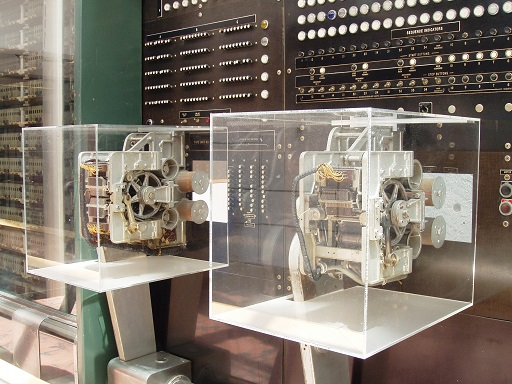
\includegraphics[scale=0.75]{HarvardMarkI.jpg}
\end{center}
\caption{računar Harvard Mark I}
\label{fig:HM1}
\end{figure}

\subsection{Oporavak kompanije od rata i uspon u svetu računarstva}%KOD UNIVACA IDE CITA(valjda)
Iako je kompanija izbacila svoj prvi kompjuter godinu dana nakon što je izbačen čuveni UNIVAC\cite{univac} računar 1951. godine, u roku od 5 godina IBM je obuhvatao 85\% tržista. Direktor UNIVAC-a je se žalio:``Nije od velikog značaja kada napravite bolji proizvod u koliko drugi imaju pet puta više prodavača nego vi``. Kada je preminuo direktor kompanije, Votson Senior, njegovu poziciju 1952. godine zauzeo je njegov najstariji sin, Votson Junior(eng.~{\em Thomas J. Watson Jr.}). Nakon smenjivanja direktora, kompanija je bila u sred tehnološke revolucije, neverovatno brzo su se razvijali elektronski računari, magnetne trake, kao i samo programiranje. Votson Junior i njegovi saradnici u okviru kompanije pitali su se da li su dorasli izazovu vođenja IBM-a nakon što je Votson Senior preminuo. Votson Junior je na to pitanje odgovorio drastično izvršio promene u organizaciji kompanije, što je olakšalo dalje proširivanje u svetu računarstva.

\section{Zlatno doba IBM-a}%slike citati fusnote literatura
Tokom 1960ih, kompanija IBM je uspela da hrabrim i promišljenim odlukama, i inovativnim idejama ovlada tržištem biznis računara. Vođena iskusnim i talentovanim rukovodstvom%fusnota predsednik?
, kompanija je prešla sa proizvodnje pisaćih mašina i bušenih kartica na proizvodnju digitalnih računara, u kojima je videla svoju budućnost i potencijal za dalji razvoj.
Sa svojim revolucionarnim patentima i idejama ponovo se našla na čelu industrije, i nastavila je da je vodi i usmerava, postavljajući standarde koji su opstali i do danas.\\
Sa čak 70\% udela računara dominirala je tržištem, %antitrust?
a svoj domet uveliko je proširila i na ostatak sveta. Zarada kompanije se uvećala čak pet puta i iznosila je 7,5 milijardi dolara, dok se broj zaposlenih više nego duplirao i iznosio je preko 250 hiljada. %TODO referenca
\subsection{Važni pronalasci} 
Za prethodan uspeh zaslužne su pre svega dve stvari, porodica računara \emph{Sistem/360}  i zasebna proizvodnja softvera i hardvera.
\subsubsection*{Sistem/360}Sistem/360 je familija mejnfrejm (eng.~{\em mainframe}) računara srednje jačine. To je bio najznačajniji proizvod kompanije do tada. Pored toga što je bio veliki uspeh u prodaji ovaj sistem je važan jer se prvi put javlja lanac računara koji su međusobno kompatabilni.
Računari su bili iste arhitekture što je omogućilo razmenu softvera kao i periferijskih uređaja i kostimizaciju. Korisniku su na raspolaganju bile verzije različite brzine procesora i količine memorije. \\%konkretno?
Mnogo su sa oprezom gledali na ovaj korak ka kompatabilnim računarima za generalnu upotrebu, međutim pokazalo se da je IBM još jednom napravio ispravnu odluku i pokrenuo novi trend u industriji.%Forbs 5mil gabmle fusnota?
\subsubsection*{Odvajanje prodaje i proizvodnje programa i računara} Ova odluka je bila velika i neočekivana prekretnica dotadašnjeg načina poslovanja i prodaje računara. Prethodno je računar podrazumevano dolazio u paketu sa svim potrebnim programima i sa njima činio nerazdvojivu celinu.\\
Razdvajanjem ova dva dela IBM je u potpunosti promenio pogled korisnika i industrije na aplikativni softver. Ovom odlukom pokrenuta je multimilionska industrija razvoja softvera i poboljšan njegov kvalitet i raznovrsnost. 
\subsubsection*{Nove vrste memorije}
IBM je zaslužan za pronalazak kartica sa magnetnom trakom. Takve kartice su našle veliku primenu i koriste se i danas (npr. kartice za zaposlene, ili bankarske kartice). One su usvojene kao standard, i koristile su se uz IBM-ovu mašinu za očitavanje (preteča bankarskog automata).\\
Još jedna upotreba tehnologije magnetnih traka jeste i izum \emph{floppy disk}-a koji je zbog svoje prenosivosti ubrzo postao uobičajno skladište ličnih računara.\\ Takođe, povezivanjem magnetnog skladišta sa pisaćom mašinom nastala primitivna verzija današnje obrade dokumenta.\\
Pored ovoga IBM je razvio i brzu memoriju sa jednoćelijskim tranzistorima danas poznatiju kao DRAM (eng.~{\em Dynamic Random Access Memory}).%eng?
\\ \\
IBM je u doprineo i sletanju čoveka na mesec. Njihova tehnologija koristila se za razna izačunavanja putanja, a i direktno u letelici za navođenje leta.\\
U okviru IBM-a razvijeni su i prva relaciona baza podataka, rana vrsta protokola za komunikaciju preko mreže, kao i čitač i sistem bar-kodova.
%
\section{Razvoj ličnih računara i pad IBM-a}
\subsection{Propust u razvoju minikompjutera}
Nakon tri decenije velikog uspeha, rasta i napretka IBM se našao u nepogodnoj situaciji i polako počeo da gubi na značaju. %
Sve više konkurencije počelo je da preti IBM-u, dok se tržište menjalo i udaljavalo od onog u kom je IBM blistao. Dodatno, predsednik kompanije, koji je u velikoj meri bio zaslužan za prethodni uspeh, morao je da napusti svoju poziciju.\\%kad ko zasto i ko ga je nasledio fusnota?
Kompanija koja je prethodno imala monopol nad tržištem propustila je novi trend biznis računara, \emph{minikompjutere}, i dozvolila ostalim kompanijama da je zamene. Dok je 1970ih imala oko 60\% svih računara na tržištu, 1980ih je ta brojka pala na 30\%. %fusnota okoncan antitrust, i citat
\subsection{Uspešna proizvodnja ličnih računara}
Međutim to nije bio kraj za IBM. Nazirao se sledeći veliki period u industriji koji IBM nije imao nameru da propusti. Sa starih mejnfrejm računara se prešlo na miniračunare, a zatim je usledilo i doba ličnih kompjutera. \\Pored malog zakašnjenja, IBM je uspeo da se povrati i uspešno uključi u proizvodnju ličnih računara.\\ Prvobitno izbacuje model IBM 5100 koji prestavlja ranu, prelaznu verziju prenosivog računara, a zatim u prodaju pušta i IBM PC. To je bio računar skromnih sposobnosti, ali je imao sve funkcionalnosti potrebne korisniku. Uz prepoznatljiv brend, dobar marketing i razvijenu mrežu trgovaca, IBM PC je uspeo da vrati kompaniju na noge, dajući joj 1985. godine čak i status najprofitabilnije kompanije.%izvor?
 \\Nedugo nakon toga kompanije iznenađuje sve sa svojim modelom IBM PC AT koji je imao dobre performanse i veoma nisku cenu. 
\subsection{Pogrešne odluke}
Ipak nakon kratkog povratka kompanija nailazi na još veći pad od kog se nikad neće potpuno oporaviti. % 
Da bi ubrzala proces proizvodnje računara kompanija IBM je prekršila svoje pravilo da sve komponente proizvodi sama. Odluka da se za razvoj operativnog sistema osloni na kompaniju Microsoft, a mikroprocesore nabavlja od kompanije Intel biće fatalna po IBM. Obe kompanije počinju da se razvijaju i nadrastaju IBM, preuzimajući njen prethodni monopol. Pritom je konkurencija sada imala mogućnost da pravi kompatabilne kopije i time oslabi brend IBM-a i njegov značaj.  \\
Usled propuštenih prilika i nespretnih odluka, kompanija narednih godina trpi velike gubitke. Od 1991. do 1993. IBM prijavljuje gubitke od čak 16 milijardi dolara. Pored Majkrosofta i Intela, kompanija Seagate joj preotima proizvodnju \emph{hard diskova}, HP štampača, Oracle baza podataka, a Dell računara. \\ 
Kako bi se povratila, prinuđena je da rasproda sva neključna poslovanja, smanji broj zaposlenih i prilagodi se novoj situaciji. Uspeva da opstane skroz menjajući fokus sa hardvera na softverska rešenja i usluge.


\begin{figure}[!hb]
\centering
\begin{minipage}{.5\textwidth}
  \centering
  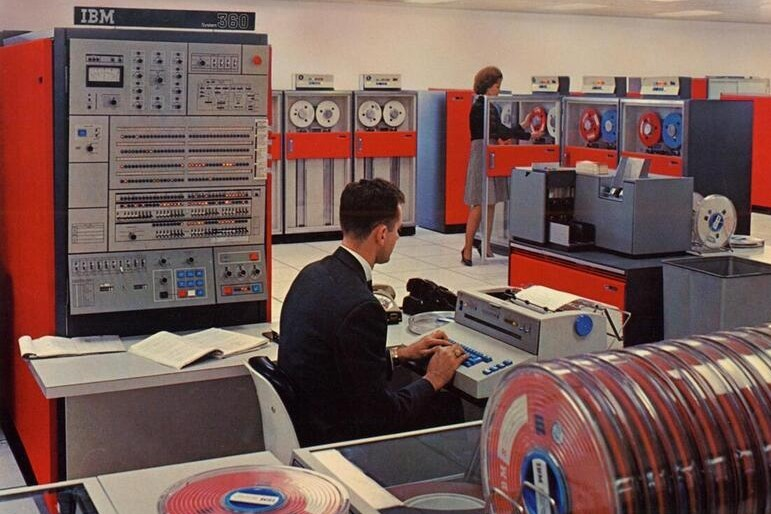
\includegraphics[width=.6\linewidth]{sys360.jpg}
  \captionof{figure}{Sistem 360}
  \label{fig:S360}
\end{minipage}%
\begin{minipage}{.5\textwidth}
  \centering
  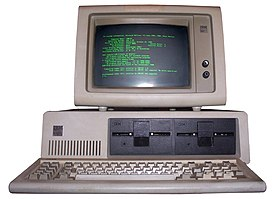
\includegraphics[width=.6\linewidth]{ibmpc.jpg}
  \captionof{figure}{računar IBM PC}
  \label{fig:IBMPC}
\end{minipage}
\end{figure}

\section{Kompanija IBM u sadašnjosti i budućnosti}
Kompanija IBM danas nije isto što i kompanija IBM pre 30 godina. Naime, pre 30 godina IBM bila je jedna od najmoćnijih u svetu tehnologije. Prodavali su svoje PC računare i u tome su bili veoma uspešni.
Danas, IBM više nema licencu za svoje PC računare, jer su ih prodali kineskoj kompaniji \textbf{Lenovo}\cite{lit1}. I oni veoma uspešno plivaju u prodaji laptop računara, pre svega serije \textbf{ThinkPad} koja je originalno napravljena od strane IBM-a. Iako je kompanija IBM godinama bila dominantna, danas više teži ka propadanju. Međutim neki analitičari smatraju da je moguć povratak u visoki rang, zajedno sa njihovom dugogodišnjom konkurencijom, jer se trenutno bave cloud servisima i procene su da je moguće da napreduju u periodu između 2022. i 2024. godine.

\begin{primer}
Najveća konkurencija su kompanije Google, Microsoft i Amazon.
\end{primer}

Velika greška ove kompanije je pre svega kasno izbacivanje proizvoda na berzu, do toga je dolazilo iz više razloga. Najviše zbog:

\begin{itemize}
\item detaljnih analiza i testiranja proizvoda
\item nepoznavanja marketa i berze
\item nesuglasica između kolega u kompaniji...
\end{itemize}

IBM se bavi i veštačkom inteligencijom(eng.~{\em Artificial intelligence}). Najpoznatiji projekat, koji ih je i stavio na loš glas u svetu tehnologije, je robot Vatson(eng.~{\em Watson}) za koga je zamisao bila da može da odgovori na sva postavljena pitanja i namena je bila u medicinske svrhe. Međutim, ispostavilo se da robot nije radio ono što su oni zamislili i da je samo mogao da razume reči i da ih čita, i uprkos kritikama od strane stručnih ljudi, IBM odlučuje da Vatson-a izbaci u prodaju. Prodaja nije prošla dobro i to je najveći neuspeh ove kompanije. Odlučuju se da ga prodaju 2022. godine.

Kompanija se 2021. godine deli na dve dela, kao strategija za napredovanje. Odvaja se odeljenje Managed Infrastructure Services, a ostatak kompanije će imati fokus na hibridnu cloud platformu, kao i implementaciju tehnologija koje se tiču veštačke inteligencije.


\begin{table}[h!]
\begin{center}
\caption{Zarada kompanije IBM u prethodnih 5 godina i broj zaposlenih. \cite{tabela}}
\begin{tabular}{|c|c|c|c|c|} \hline
Year& Net income in mil.USD& Price per share in USD& Employees \\ \hline
2017	&5,753		&149.76	&366,600\\ \hline
2018	&8,723		&139.90	&350,600\\ \hline
2019	&9,400		&126.85	&352,600\\ \hline
2020	&5,590	  &125.88	&345,900\\ \hline
2021	&5,743		&133.66	&282,100\\ \hline
\end{tabular}
\label{tab:tabela1}
\end{center}
\end{table}

\section{Zaključak}
Kompanija IBM je i dalje aktivna i bavi se proizvodnjom računarskog hardvera, softvera, uslugama, hostingom i konsaltingom. Iako više nije toliko dominantna na tržištu, ostavila je veliki trag u razvoju računarstva. 

\addcontentsline{toc}{section}{Literatura}
\renewcommand{\refname}{Literatura}
\begin{thebibliography}{10}
\bibliographystyle{unsrt}
\bibitem{istorija} History of IBM at:\\ \url{https://www.ibm.com/ibm/history/history/history_intro.html}
\bibitem{univac} About Univac at: \url{https://www.britannica.com/technology/UNIVAC}
\bibitem{lit1} What happend to IBM?\\ \url{https://www.thecoldwire.com/what-happened-to-ibm}
\bibitem{tabela} Wikipedia \url{https://en.wikipedia.org/wiki/IBM} %WIKI?
\bibitem{ibm} About IBM at: \url{https://www.ibm.com/academic/home}
\bibitem{knjiga} Predrag Janičić, Filip Marić: Programiranje 1, Matematički fakultet, Beograd, 2015.
%https://history-computer.com/ibm-history/
%https://www.thoughtco.com/ibm-timeline-1992491
%https://www.ibm.com/ibm/history/history/decade_1900.html
%https://en.wikipedia.org/wiki/History_of_IBM
\end{thebibliography}
\end{document}

